\documentclass[a4paper,12pt]{article} % тип документа
\usepackage[margin=1in]{geometry} % Поля

%  Русский язык
\usepackage[warn]{mathtext}
\usepackage[T2A]{fontenc}			% кодировка
\usepackage[utf8]{inputenc}			% кодировка исходного текста
\usepackage[english,russian]{babel}	% локализация и переносы
% Математика
\usepackage{amsmath,amsfonts,amssymb,amsthm,mathtools} 
\usepackage{wasysym}
%%%
\usepackage{graphicx}

\usepackage{tabularx}
\usepackage[table,xcdraw]{xcolor}

\usepackage{gensymb} % знак градуса
\usepackage{enumitem} % изменить список enumerate
\usepackage{placeins} % \FloatBarrier

\renewcommand{\thesection}{\Roman{section}} 
\renewcommand{\thesubsection}{\roman{subsection}}


\begin{document}

\newcolumntype{Y}{>{\centering\arraybackslash}X} %new tabularx


%титул

\begin{center}
{\LARGE Московский Физико-Технический Институт}
\\
{\large Физтех-школа электроники, фотоники и молекулярной физики }
\\
\vspace{8cm}
{\LARGE Отчёт по лабораторной работе:}
\\
{\Huge Электронно-оптический преобразователь} 
\\
\vspace{5cm}
\raggedright 
\hspace{8cm}{\large Выполнили работу студенты }\\
\hspace{8cm}{\large группы Б04-005:}\\
\hspace{8cm}{\large Давыдов Владислав}\\
\hspace{8cm}{\large Карташов Констанин}\\
\hspace{8cm}{\large Корнеев Николай}\\

\vspace{\fill}
\center
{\large Долгопрудный 2022}

\end{center}

\newpage


\section{Анотация}

\paragraph{Цель работы:} 
Знакомство с устройством электронно-оптического преобразователя. Получение картинки на экране ЭОП. Исследование зависимости токов в ЭОП от напряжения. Исследование условий видимости картинки на экране ЭОП.

\paragraph{Оборудование:}
\begin{itemize}
\renewcommand{\labelitemi}{$\triangleright$}
\itemsep0em
\item Электронно-оптический преобразователь,
\item Веб-камера,
\item Персональный компьютер.
\end{itemize}

\subsection{Устройство электронно-оптического преобразователя}

\paragraph{} ЭОП состоит из:

\begin{itemize}
\item Фотокатода, который преобразует падающий свет в поток электронов.
\item Микроканальной пластинки, усиливающей поток электронов.
\item Электростатической линзы, фокусирующей поток электронов на экране.
\item Экрана, преобразующего поток электронов в световое излучение.
\end{itemize}

\begin{figure}[h]
\centering
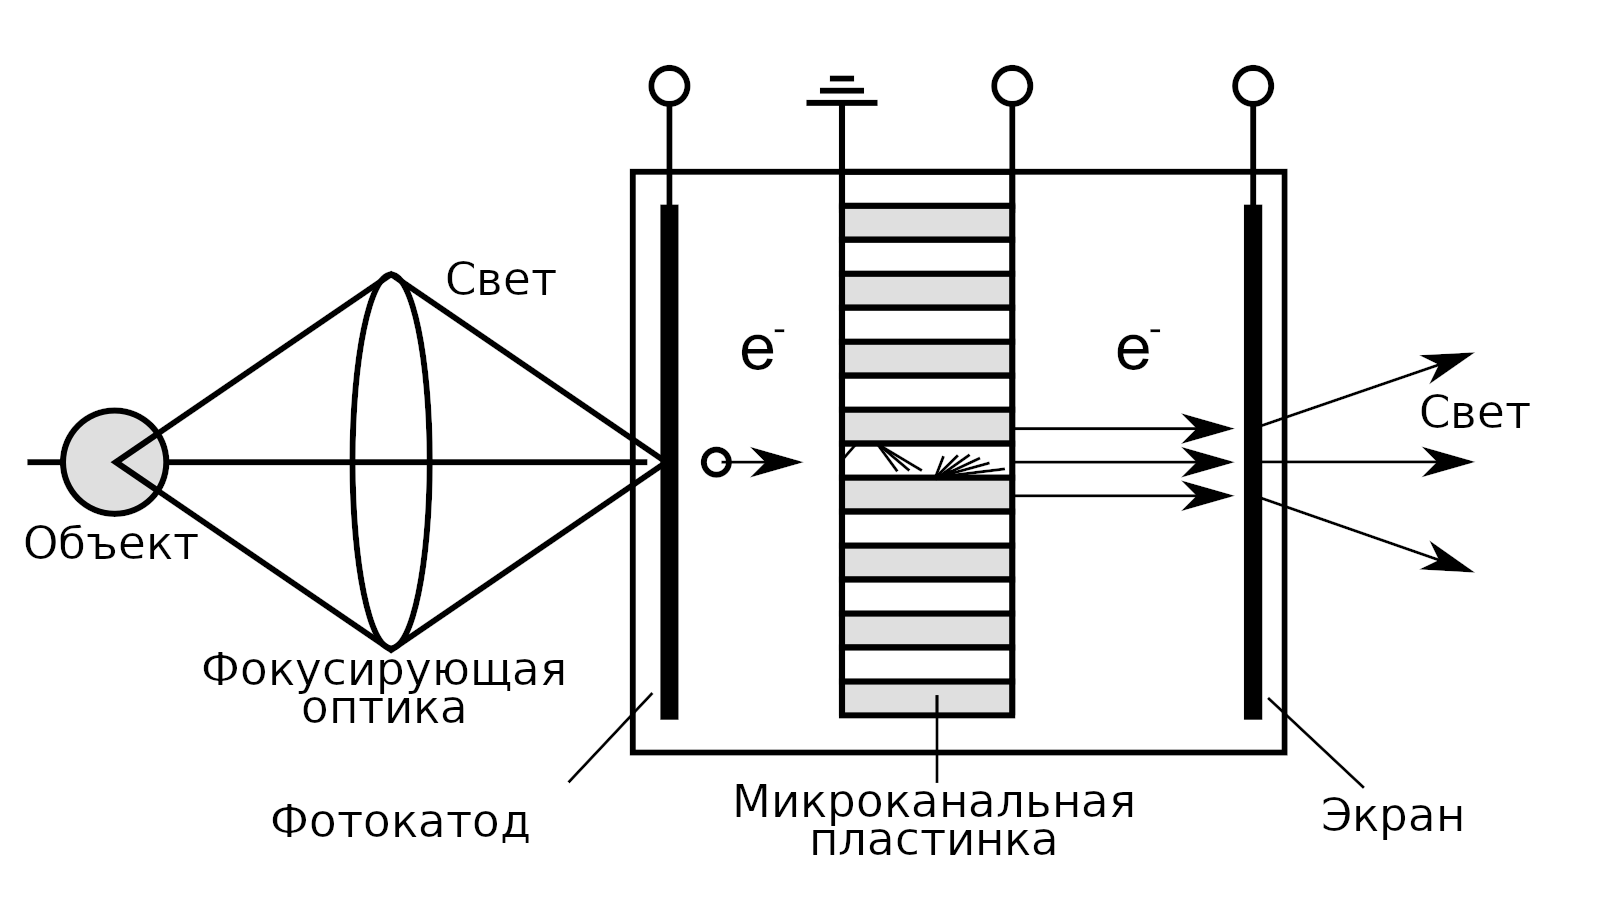
\includegraphics[width=0.7\textwidth]{setup.png}
\caption{Устройство ЭОП}
\label{fig:setup}
\end{figure}


\medskip\hrule\medskip

\section{Проведения измерений}

\subsection{ВАХ электронно-оптического преобразователя}

\paragraph{} Для переменных значений $U_\text{катод}$, $U_\text{МКП}$, $U_\text{экран}$ сними вольт-амперную характеристику ЭОП. Полученные данные представлены в табл. \ref{tab:kat}, \ref{tab:mkp}, \ref{tab:ekr}. По этим данным можно сделать следующие выводы:

\begin{enumerate}
\item $I_\text{катод}$ и $I_\text{экран}$ практически равны нулю.
\item При переменном $U_\text{катод}$ незначительно увеличиваются $I_\text{анод}$ и $I_\text{экран}$.
\item При переменном $U_\text{МКП}$ меняется $I_\text{МКП}$.
\item При переменном $U_\text{экран}$ ничего не меняется.
\end{enumerate}

\begin{table}[h]
\centering
\begin{tabular}{|l|r|r|r|r|r|r|r|r|r|}
\hline
$U_\text{катод}$, В  & 0.91 & 1.30 & 1.70 & 2.11 & 2.50 & 2.90 & 3.28 & 3.69 & 4.11 \\ \hline
$I_\text{катод}$, мА & 0    & 0    & 0    & 0    & 0    & 0    & 0    & 0    & 0    \\ \hline
$I_\text{МКП}$, мА   & 8.86 & 8.85 & 8.85 & 8.85 & 8.85 & 8.85 & 8.85 & 8.85 & 8.85 \\ \hline
$I_\text{экран}$, мА & 0    & 0    & 0    & 0    & 0    & 0.05 & 0.06 & 0.08 & 0.08 \\ \hline
$I_\text{анод}$, мА  & 4.48 & 4.48 & 4.48 & 4.48 & 4.50 & 4.51 & 4.52 & 4.53 & 4.53 \\ \hline
\end{tabular}
\caption{Токи при переменном $U_\text{катод}$ ( $U_\text{МКП} = 2.01$ В, $U_\text{экран} = 2.95$ В)}
\label{tab:kat}
\end{table}

\begin{table}[h]
\centering
\begin{tabular}{|l|r|r|r|r|r|r|r|}
\hline
$U_\text{МКП}$, В    & 0.32 & 0.60 & 0.90 & 1.20 & 1.50 & 1.80 & 2.00 \\ \hline
$I_\text{катод}$, мА & 0    & 0    & 0    & 0    & 0    & 0    & 0    \\ \hline
$I_\text{МКП}$, мА   & 1.33 & 2.53 & 3.70 & 5.00 & 6.34 & 7.66 & 8.80 \\ \hline
$I_\text{экран}$, мА & 0    & 0    & 0    & 0    & 0    & 0    & 0    \\ \hline
$I_\text{анод}$, мА  & 0.66 & 1.27 & 1.87 & 2.54 & 3.22 & 3.89 & 4.49 \\ \hline
\end{tabular}
\caption{Токи при переменном $U_\text{МКП} $ ( $U_\text{катод} = 3$ В, $U_\text{экран} = 2.95$ В)}
\label{tab:mkp}
\end{table}

\begin{figure}
\centering
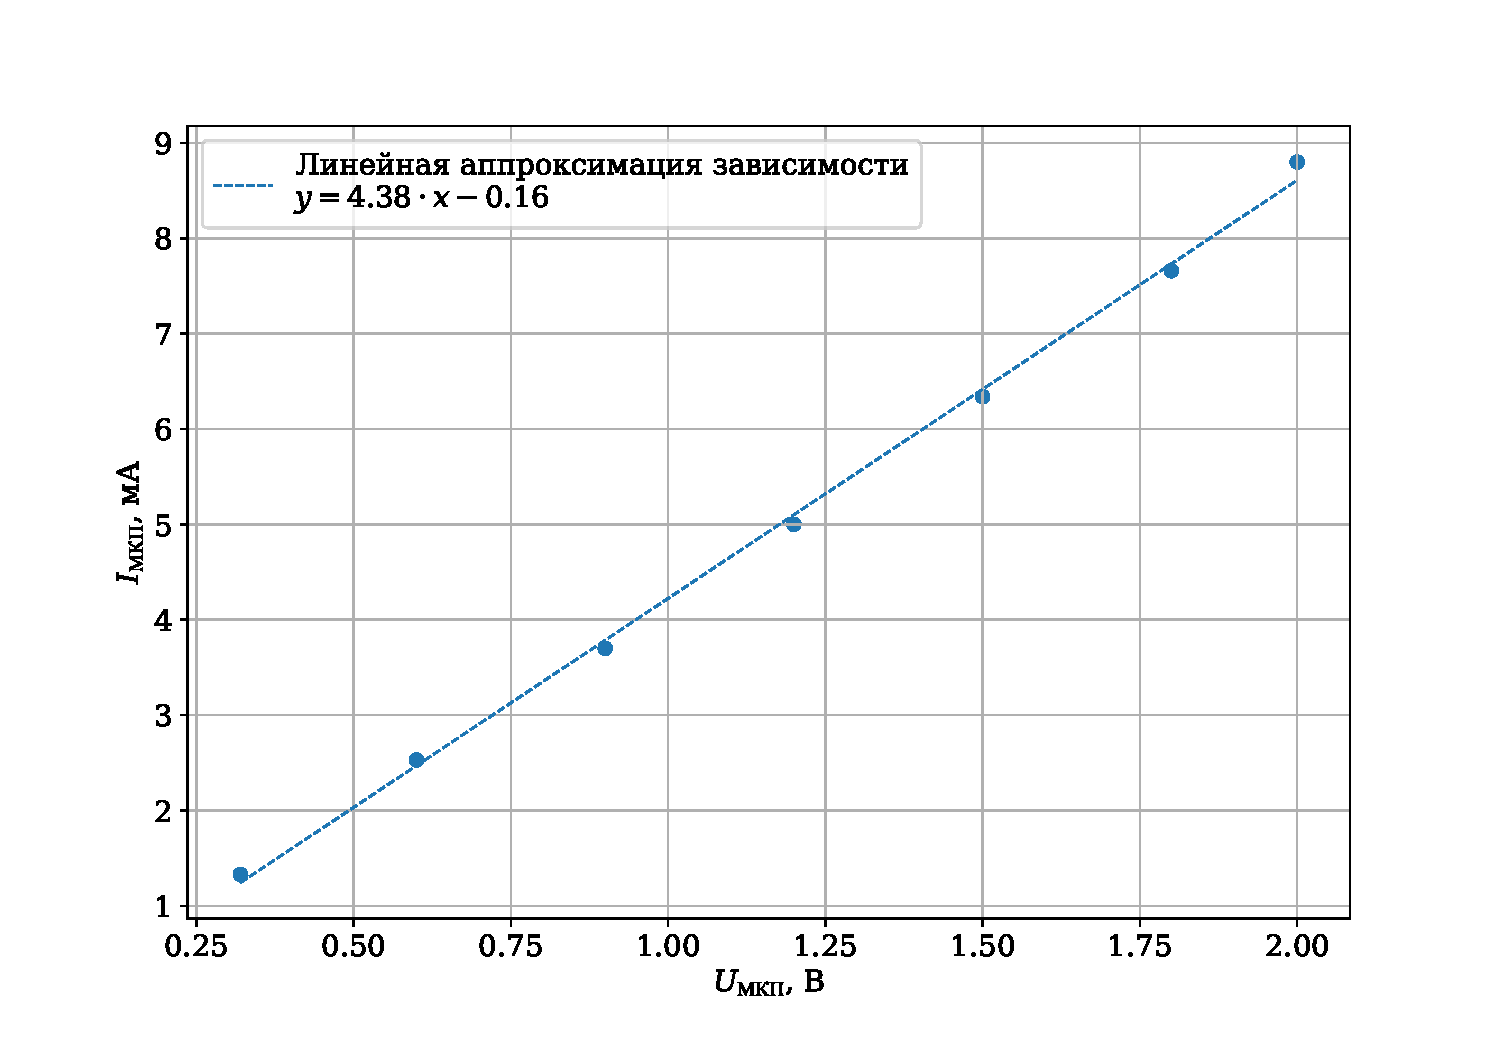
\includegraphics[width=\textwidth]{plot2.pdf}
\caption{Зависимость $I_\text{МКП}$ от $U_\text{МКП}$ соответствующая табл. \ref{tab:mkp}}
\end{figure}

\begin{table}[h]
\centering
\begin{tabular}{|l|r|r|r|r|r|r|r|r|}
\hline
$U_\text{экран}$, В  & 0.82 & 1.10 & 1.40 & 1.71 & 2.00 & 2.30 & 2.60 & 2.90 \\ \hline
$I_\text{катод}$, мА & 0    & 0    & 0    & 0    & 0    & 0    & 0    & 0    \\ \hline
$I_\text{МКП}$, мА   & 8.75 & 8.76 & 8.76 & 8.80 & 8.79 & 8.79 & 8.79 & 8.79 \\ \hline
$I_\text{экран}$, мА & 0.05 & 0.04 & 0.05 & 0.05 & 0.05 & 0.05 & 0.05 & 0.05 \\ \hline
$I_\text{анод}$, мА  & 4.46 & 4.46 & 4.47 & 4.46 & 4.47 & 4.47 & 4.47 & 4.47 \\ \hline
\end{tabular}
\caption{Токи при переменном $U_\text{экран} $ ( $U_\text{катод} = 3$ В, $U_\text{МКП} = 2$ В)}
\label{tab:ekr}
\end{table}

\subsection{Исследование видимости на экране}

\paragraph{} При фиксированном $U_\text{экран}$ снимем зависимость $U_\text{катод}$ от $U_\text{МКП}$ при предельной видимости картинки на экране. Результаты измерений представлены в табл. \ref{tab:my-table}. По данным построим график (рис. \ref{fig:plot-vis}).

\paragraph{} Сделаем аппроксимацию к точками на графике пользуясь методом наименьших квадратов. Получим кривую $y = \frac{1.03 \cdot x}{x - 0.79}$ (рис. \ref{fig:approx}).

\begin{table}[h]
\centering
\begin{tabular}{|l|r|r|r|r|r|r|r|}
\hline
$U_\text{катод, Влад}$, В & 3.05 & 2.55 & 2.1  & 1.97 & 1.9 & 1.76 & 1.65 \\ \hline
$U_\text{МКП, Влад}$, В   & 1.4  & 1.5  & 1.6  & 1.7  & 1.8 & 1.9  & 2    \\ \hline
$U_\text{катод, Коля}$, В & 3.1  & 2.66 & 2.25 & 2.09 & 1.9 & 1.8  & 1.72 \\ \hline
$U_\text{МКП, Коля}$, В   & 1.4  & 1.5  & 1.6  & 1.7  & 1.8 & 1.9  & 2    \\ \hline
\end{tabular}
\caption{Зависимость напряжений катода и МКП при предельной видимости}
\label{tab:my-table}
\end{table}

\begin{figure}[h]
\centering
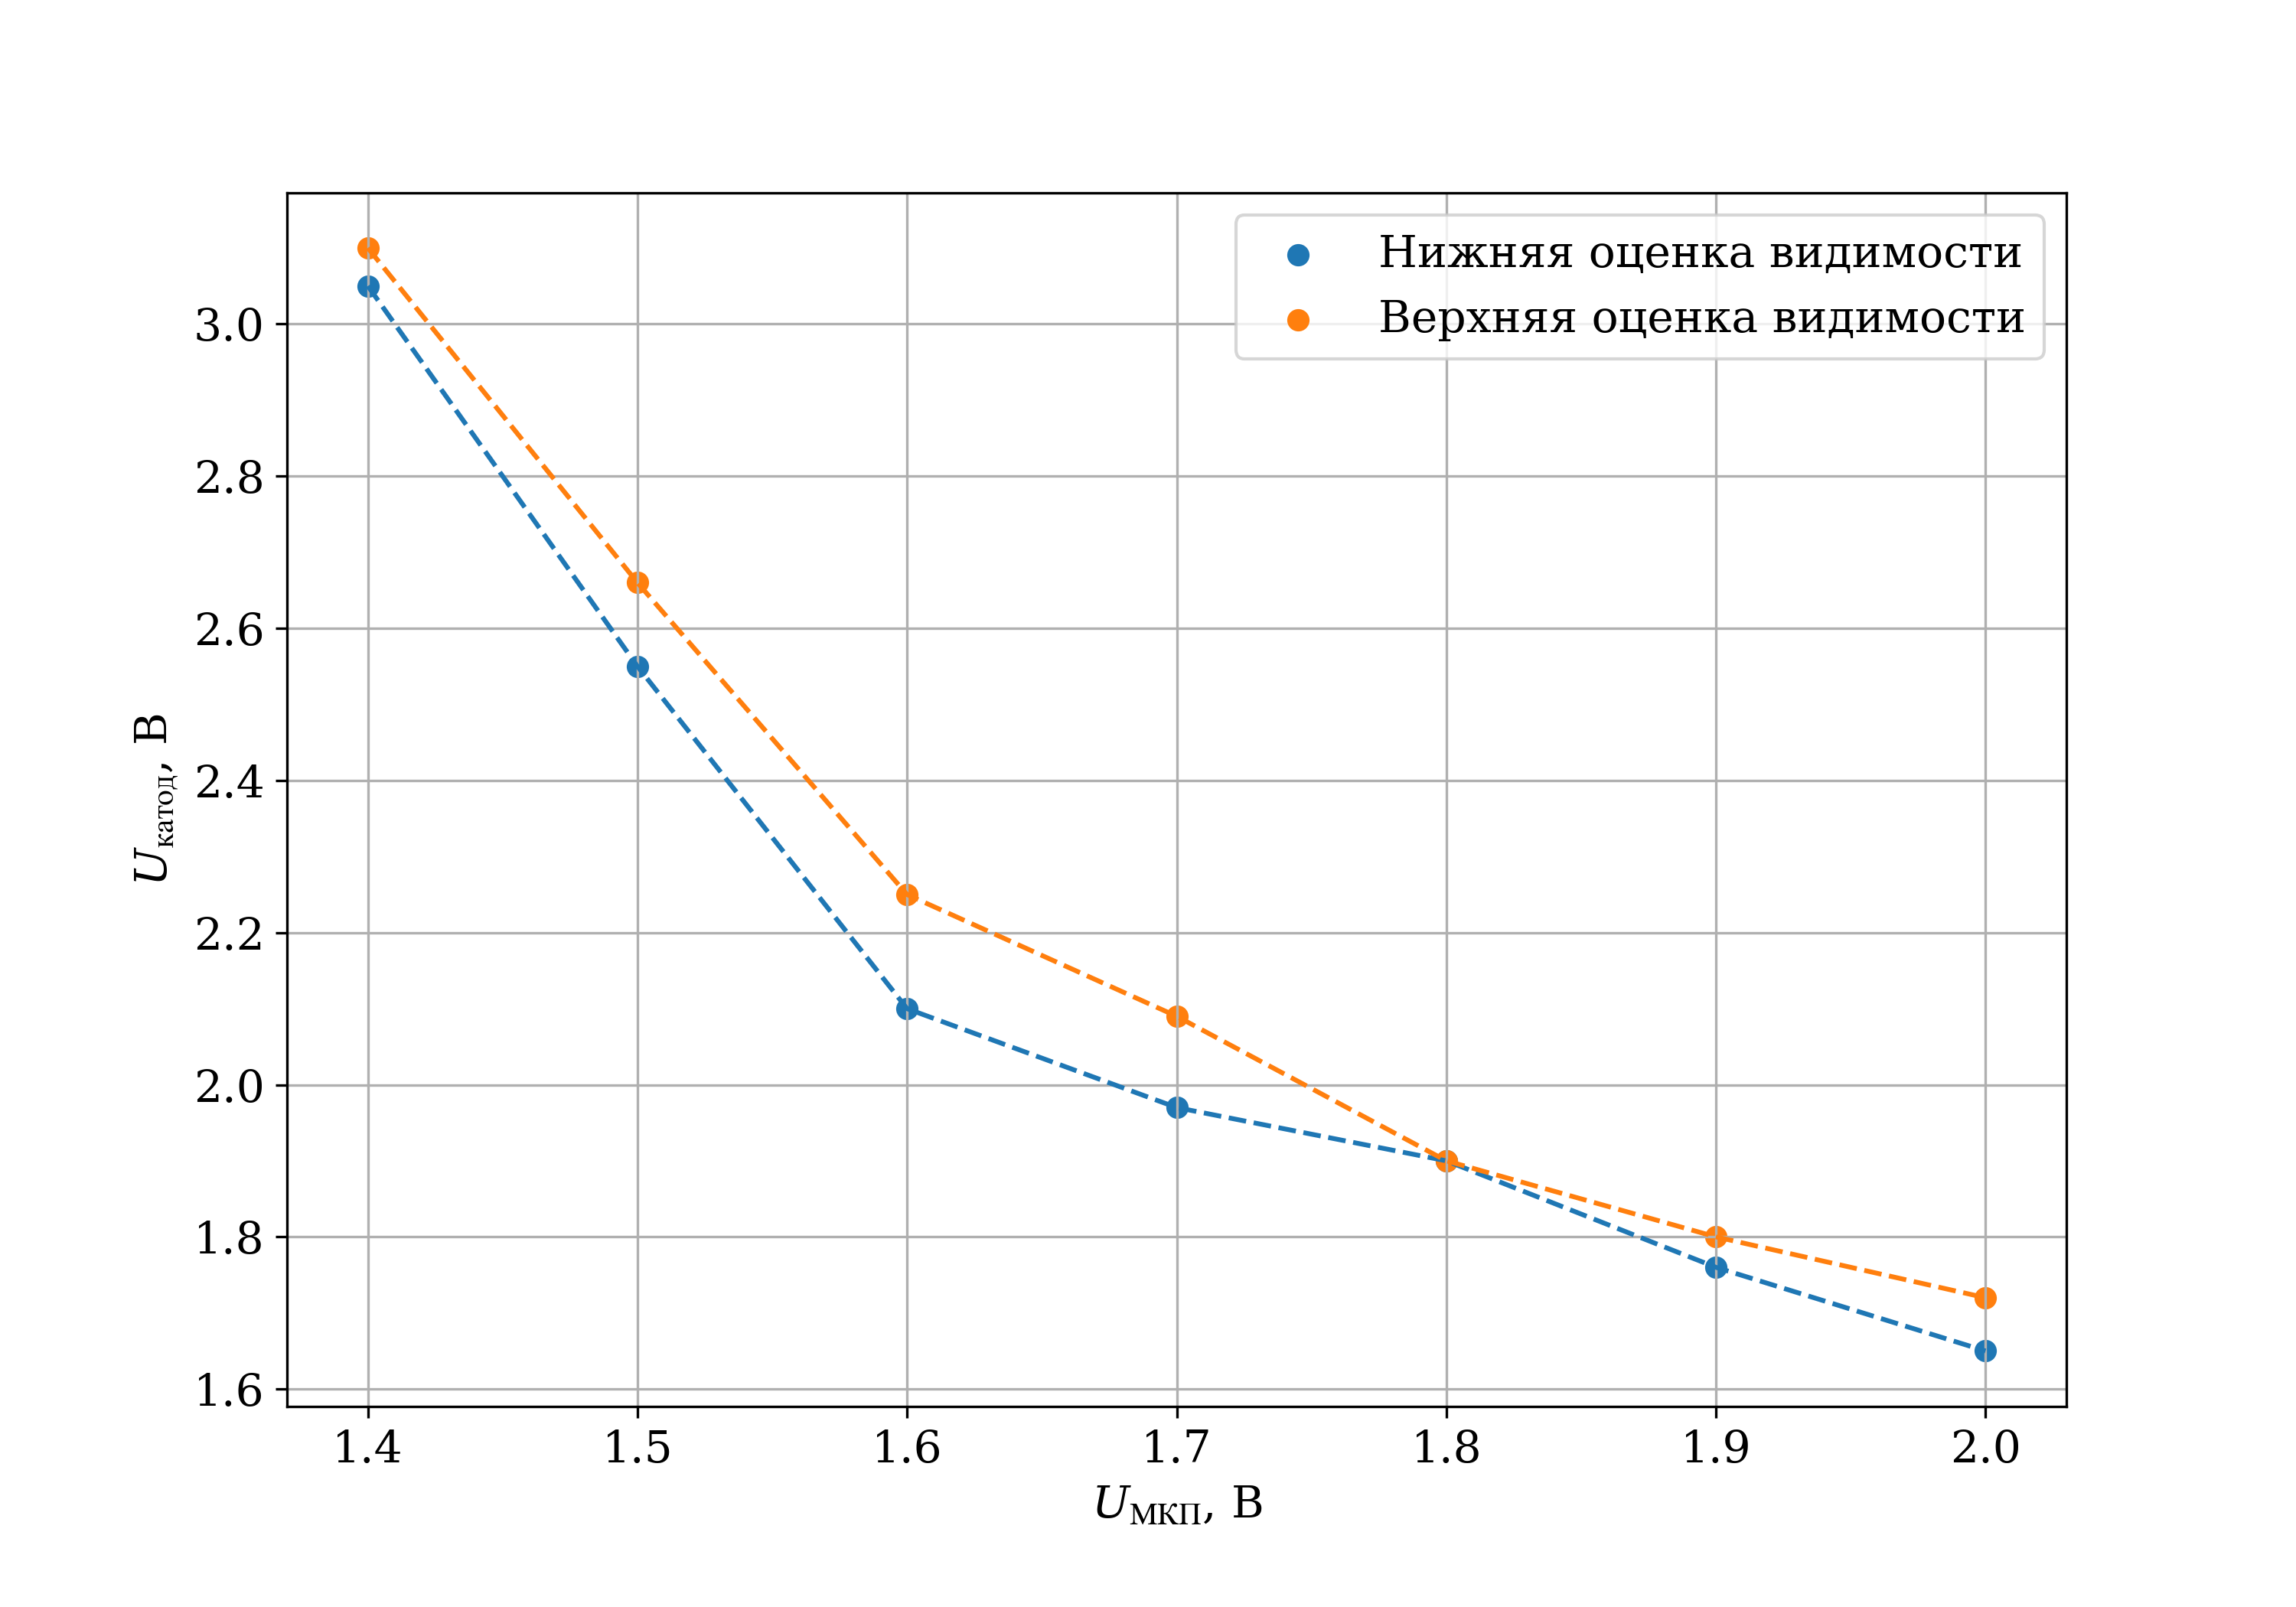
\includegraphics[width=\textwidth]{plot_vis.png}
\caption{График зависимости $U_\text{катод}$ от $U_\text{МКП}$ при одинаковой видимости}
\label{fig:plot-vis}
\end{figure}

\begin{figure}
\centering
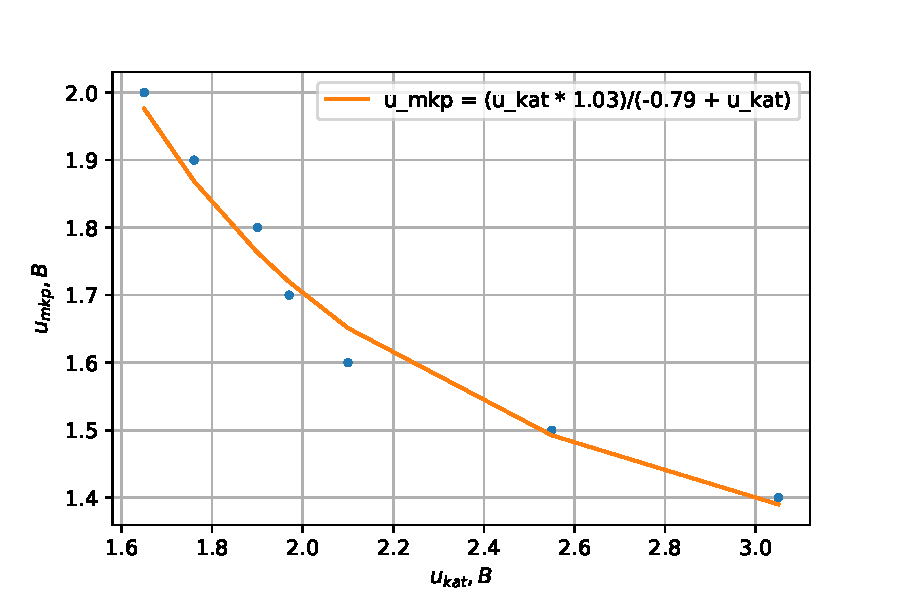
\includegraphics[width=\textwidth]{goodgame.pdf}
\caption{Аппроксимация зависимости $U_\text{МКП}$ от $U_\text{катод}$}
\label{fig:approx}
\end{figure}


\end{document}
